%%
%% Copyright 2007, 2008, 2009 Elsevier Ltd
%%
%% This file is part of the 'Elsarticle Bundle'.
%% ---------------------------------------------
%%
%% It may be distributed under the conditions of the LaTeX Project Public
%% License, either version 1.2 of this license or (at your option) any
%% later version.  The latest version of this license is in
%%    http://www.latex-project.org/lppl.txt
%% and version 1.2 or later is part of all distributions of LaTeX
%% version 1999/12/01 or later.
%%
%% The list of all files belonging to the 'Elsarticle Bundle' is
%% given in the file `manifest.txt'.
%%

%% Template article for Elsevier's document class `elsarticle'
%% with numbered style bibliographic references
%% SP 2008/03/01
%%
%%
%%
%% $Id: elsarticle-template-num.tex 4 2009-10-24 08:22:58Z rishi $
%%
%%
%%\documentclass[preprint,12pt,3p]{elsarticle}

%% Use the option review to obtain double line spacing
%%\documentclass[preprint,review,12pt]{elsarticle}

%% Use the options 1p,twocolumn; 3p; 3p,twocolumn; 5p; or 5p,twocolumn
%% for a journal layout:
%% \documentclass[final,1p,times]{elsarticle}
%% \documentclass[final,1p,times,twocolumn]{elsarticle}
%% \documentclass[final,3p,times]{elsarticle}
\documentclass[final,3p,times,twocolumn]{elsarticle}
%% \documentclass[final,5p,times]{elsarticle}
%% \documentclass[final,5p,times,twocolumn]{elsarticle}

%% if you use PostScript figures in your article
%% use the graphics package for simple commands
%% \usepackage{graphics}
%% or use the graphicx package for more complicated commands
%% \usepackage{graphicx}
%% or use the epsfig package if you prefer to use the old commands
%% \usepackage{epsfig}


%% The amssymb package provides various useful mathematical symbols
\usepackage{blindtext, graphicx, amsmath, algorithm, algpseudocode, pifont, algcompatible, comment, layout, amsthm, amssymb}
\usepackage{enumitem}   
\usepackage{eso-pic}
\usepackage{booktabs}
\usepackage{float}
%% The amsthm package provides extended theorem environments
%% \usepackage{amsthm}
\renewcommand{\qedsymbol}{$\blacksquare$}

\usepackage[utf8]{inputenc}
\usepackage[english]{babel}
\usepackage{hyperref} 
\hypersetup{ colorlinks=true, linkcolor=black, filecolor=black, urlcolor=cyan, }

\usepackage{caption}
\captionsetup{justification=raggedright, singlelinecheck = false}
\captionsetup[table]{labelformat=simple, labelsep=newline}
\captionsetup[figure]{labelformat=simple, labelsep=period}


%% The lineno packages adds line numbers. Start line numbering with
%% \begin{linenumbers}, end it with \end{linenumbers}. Or switch it on
%% for the whole article with \linenumbers after \end{frontmatter}.
%% \usepackage{lineno}

%% natbib.sty is loaded by default. However, natbib options can be
%% provided with \biboptions{...} command. Following options are
%% valid:

%%   round  -  round parentheses are used (default)
%%   square -  square brackets are used   [option]
%%   curly  -  curly braces are used      {option}
%%   angle  -  angle brackets are used    <option>
%%   semicolon  -  multiple citations separated by semi-colon
%%   colon  - same as semicolon, an earlier confusion
%%   comma  -  separated by comma
%%   numbers-  selects numerical citations
%%   super  -  numerical citations as superscripts
%%   sort   -  sorts multiple citations according to order in ref. list
%%   sort&compress   -  like sort, but also compresses numerical citations
%%   compress - compresses without sorting
%%
%% \biboptions{comma,round}

% \biboptions{}
\newtheorem{theorem}{Theorem}
\newtheorem{lemma}{Lemma}
\newtheorem{definition}{Definition}

\journal{ICT Express}

%\newcommand\AtPagemyUpperRight[1]{\AtPageLowerRight{%
%\put(\LenToUnit{0.8\paperwidth},\LenToUnit{0.9\paperheight}){#1}}}
%\AddToShipoutPictureFG{
%  \AtPagemyUpperRight{{\includegraphics[width=.5cm,keepaspectratio]{logo.png}}}
%}%
%\newcommand\AtPagemyUpperLeft[1]{\AtPageLowerLeft{%
%\put(\LenToUnit{0.85\paperwidth},\LenToUnit{0.9\paperheight}){#1}}}
%\AddToShipoutPictureFG{
%  \AtPagemyUpperLeft{{\includegraphics[width=1.0cm,keepaspectratio]{logo2.jpg}}}
%}%
\begin{document}

\begin{frontmatter}

\title{A Hybrid Approach of ConvLSTM-DT and GPT-4 for Real-time Anomaly Detection Decision Support in Edge-Cloud Environments}
%\author{Author’s Full Name 1\corref{cor1}, Author’s Full Name 2, Author’s Full Name 3}
\author{Radityo Fajar Pamungkas}
\ead{radityofajar@gmail.com}

\author{Ida Bagus Krishna Yoga Utama}
\ead{idabaguskrishnayogautama@gmail.com}

\author{Khairi Hindriyandhito}
\ead{khairihindri@gmail.com}

\author{Yeong Min Jang\corref{cor1}}
\ead{yjang@kookmin.ac.kr}
\address{Department of Electronics Engineering, Kookmin University, Seoul, South Korea}

\cortext[cor1]{Corresponding author}
%\ead{author1@ictexpress.com, author2@ictexpress.com, author2@ictexpress.com}

\begin{abstract}
Anomaly detection is crucial in various domains for early identification of abnormal behavior. This research introduces an innovative approach that combines prediction-based detectors with Large Language Models (LLMs) for anomaly detection, focusing on indoor air quality data from multiple sensors. The hybrid approach integrates Convolutional Long Short-term Memory with non-parametric dynamic thresholding (ConvLSTM-DT) for prediction-based anomaly detection and fine-tuned GPT-4 for generating human-understandable explanations. Each sensor parameter has its specific model for accurate predictions. Furthermore, Dynamic thresholding and continuous learning adapts to the dynamic environment, update model and setting non-parametric confidence intervals for anomaly detection in rapidly changing scenarios. The system deploys anomaly detection on the edge for reduced latency and fast detection, while LLM processing occurs on the cloud for resource optimization. The results demonstrate accurate anomaly detection and well-explained reasoning for real-time decision-making, offering a novel approach for comprehensive anomaly detection solutions in various applications. 
\\
2018 The Korean Institute of Communications and Information Sciences. Publishing Services by Elsevier B.V. This is an open access article under the CC BY-NC-ND license (http://creativecommons.org/licenses/by-nc-nd/4.0/).
\end{abstract}

\begin{keyword}
%% keywords here, in the form: keyword \sep keyword
Anomaly detection \sep Large Language Models \sep ConvLSTM-DT \sep Human-understandable explanations \sep Dynamic thresholding
%% MSC codes here, in the form: \MSC code \sep code
%% or \MSC[2008] code \sep code (2000 is the default)
\end{keyword}

\end{frontmatter}

%%
%% Start line numbering here if you want
%%
% \linenumbers

%% main text
\section{Introduction}\label{sec1}
In recent years, the rapid increase in data-driven applications and the growing complexity of modern systems have highlighted the critical significance of anomaly detection. Anomalies, often indicative of potentially harmful behavior within systems, can have long-term effects and wide-ranging consequences in various domains, such as industrial operations. Traditional anomaly detection methods, while effective to some extent, often heavily rely on expert analysis, making them resource-intensive and susceptible to human bias. This dependency on expert input can result in scalability, reliability, and consistency challenges within anomaly detection systems[1].

Furthermore, traditional anomaly detection methods based on statistical and machine learning approaches exhibit limitations, particularly when handling time-series data from multiple sensors. Anomalies in this context may be multi-dimensional and not easily characterized by conventional patterns. Consequently, traditional approaches can produce a significant number of false alarms, compromising the effectiveness and trustworthiness of anomaly detection systems[2].

In response to these challenges, this study aims to contribute to the field of anomaly detection by proposing a hybrid approach that harnesses the strength of prediction-based detector algorithms and the capabilities of Large Language Models (LLMs). This work centers on monitoring and detecting anomalies in air quality data collected from various sensors, including temperature, humidity, PM (Particulate Matter), and CO2 levels, all situated within a single indoor room environment. The ability to predict and detect anomalies in this air quality data is of paramount importance, given its profound implications for human health, particularly for those occupying the room.

The proposed hybrid approach combines Convolutional Long Short-Term Memory with non-parametric dynamic thresholding (ConvLSTM-DT) for prediction-based anomaly detection and utilizes fine-tuned GPT-4 for LLM-based explainability. This hybrid approach is essential to address the aforementioned limitations and enhance the interpretability and adaptability of anomaly detection models. It not only facilitates anomaly detection across a variety of sensors but also provides human-understandable explanations and potential solutions for addressing anomaly situations. This makes it a powerful tool for real-world implementation where swift decision-making is imperative.

\section{Literature Review}\label{sec2}
%% added tapor
Time series anomalies can be classified into five categories: global, contextual, seasonal, trends, and shapelet anomalies. Scientists are actively investigating the application of deep learning architectures for anomaly detection because of their capacity to represent data interconnections, especially in intricate structures. There are two common methods for detecting anomalies: prediction-based approaches and reconstruction-based approaches.

Malhotra et al. proposed LSTM-AD, a model that incorporates long-term memory and can detect anomalies without the need for labeled training data or unsupervised learning. Chauhan et al. introduced DeepLSTM, a method that utilizes a layered LSTM recurrent network to forecast error vectors using multivariate Gaussian distributions. Hundmand et al. developed an advanced method called LSTM-NDT for anomaly detection. This methodology utilizes non-parametric, dynamic, and unsupervised thresholding to evaluate mistakes. By combining several methodologies, LSTM-NDT achieves exceptional prediction performance.

Thill et al. proposed the integration of a Temporal Convolution Network (TCN) with an autoencoder framework (AE) for the purpose of prediction-based anomaly detection. This approach involved replacing the dense layer design with a more powerful and adaptable Convolutional Neural Network (CNN) architecture. Dai et al. created the Graph-Augmented Normalizing Flow (GANF) by incorporating graph neural networks (GNNs) in order to exploit spatial feature correlations. The GANF model serves as a powerful tool in unsupervised learning, allowing for the exploration of underlying data patterns and tackling the problem of limited labeled data.

Reconstruction-based techniques have garnered acclaim for their utilization of models such as Autoencoders (AE), LSTM-AE, and LSTM Variational Autoencoders (LSTM-VAE). These methods entail acquiring a hidden, reduced-dimensional representation to reconstruct the initial input, rendering them more suitable for detecting contextual and collective irregularities.

Gilpin's study utilized anomaly detection through explanation (ADE) by implementing reasonableness monitors that relied on anomaly detection in the simulated environment of semi-autonomous cars. This work is a groundbreaking endeavor in the field of explanatory anomaly detection, specifically focusing on providing explanations at the system level.

No work has been identified that combines both anomaly detection and Latent Logistic Regression (LLR) methods in the field of Internet of Things (IoT) and air quality monitoring. The majority of current systems for anomaly detection depend on either prediction-based or reconstruction-based techniques to identify abnormal behavior, but they lack the ability to provide thorough explanations or rationale. This paper aims to fill this void by proposing a hybrid methodology that merges prediction-based anomaly detection with LLMs to establish a reliable framework for generating explanations and reasoning in the domain of air quality monitoring in IoT devices. Therefore, the contribution for our proposed method are as follows:
%% sampe sini

Many researchers now use deep learning architecture for anomaly detection in time series due to its powerful data dependency modeling. There are two commonly used deep learning techniques: prediction-based approaches, and reconstruction-based approaches. Several prediction-based models have been developed, including the LSTM-AD that has excellent memory capabilities, and single-handedly performs anomaly detection without requiring any prior knowledge of temporal length. DeepLSTM, developed by Chauhan et al., also employs a LSTM recurrent network, offering benefits such as direct application to raw time series data, eliminating preprocessing steps. Hundmand et al.'s LSTM-NDT has superior predictive performance by integrating dynamic thresholding and anomaly scoring. Lastly, TCN-AE and GANF are used for prediction-based anomaly detection and spatial feature correlations respectively. 

Reconstruction-based approaches, on the other hand, such as Autoencoders (AE), LSTM-AE, and LSTM Variational Autoencoders (LSTM-VAE), have also been acknowledged. Unlike prediction-based anomaly detection, these approaches involve recreating the original input through a latent low-dimension representation, ideal for capturing collective anomalies. 

However, anomaly detection's integration with LLM in Internet of Things (IoT) and air quality monitoring is yet to be observed. Existing methods either rely heavily on prediction or reconstruction-based anomaly detection without providing comprehensive explanations. To fill this gap, the study introduces a hybrid approach combining prediction-based anomaly detection with LLMs within IoT systems' air quality monitoring context. 
The contributions of our proposed method are as follows: 
\begin{enumerate}
\item The hybrid approach integrating ConvLSTM-DT and Fine-tuned GPT-4 that effectively generates anomaly reasoning and possible solutions. 
\item The outlined method deploys the model in edge-cloud environments, accounting for seamless real-world edge-computing integrations. 
\item To assess the anomaly detection performance, a comparative evaluation uses machine learning anomaly detection algorithms, including Isolation Forest (iForest), One-Class Support Vector Machine (OC-SVM), Histogram-Based Outlier Score (HBOS), and Local Outlier Factor (LOF), as benchmarks for the hybrid approach.
\end{enumerate}
\section{Proposed Method}\label{sec2}

\subsection{Data Collection and Data Preprocessing}
\subsection{ConvLSTM-PBNN}
\subsection{Dynamic Thresholding}
\subsection{GPT-4 Integration}


\section{Result and Discussion}\label{sec3}

The main document with the manuscript text, figures, and tables should be prepared in an MS World or LaTeX format in English. 
The manuscript should be written in 10-point font with single line spacing on A4 sized (21.0 x 29.7 cm) paper with 1.3 cm margins on the top, bottom, right, and left. 
The standard order of sections in the manuscript is title page, abstract, introduction, system model and methods, results, discussion, references. 
Figures and tables with legends should be embedded in the proper place in the text. 
The number of all manuscript pages should be specified, starting with the title page as page 1. A single file is permitted for initial submission, but figures and tables can be uploaded separately.

\section{Conclusion}\label{sec4}
In conclusion, this research introduces a novel hybrid approach that combines prediction-based anomaly detection using Convolutional Long Short-term Memory with non-parametric dynamic thresholding (ConvLSTM-DT) and the fine-tuned GPT-4 model for Large Language Model (LLM)-based explanation generation. This hybrid approach significantly improves the interpretability and adaptability of anomaly detection models. By integrating the strengths of both prediction-based algorithms and LLMs, the model not only detects anomalies but also provides human-understandable explanations and potential solutions, making it a powerful tool for real-world applications where quick decision-making is crucial.

Furthermore, the implementation of this approach on an edge-cloud architecture enhances its performance by reducing latency and ensuring fast detection. The use of custom fine-tuning with GPT-4 tailored to the specific anomaly detection task further amplifies its accuracy. This study emphasizes the importance of domain-specific fine-tuning in achieving precise and meaningful explanations. As the field of anomaly detection continues to evolve, the presented hybrid approach, along with the use of advanced LLMs, promises to play a pivotal role in improving anomaly detection across various domains, ultimately leading to safer and more efficient operations in complex systems.

For the future work, there is significant potential for enhancing anomaly detection by incorporating commonsense reasoning trees. This addition could further bolster the accuracy and depth of anomaly reasoning and provide a more comprehensive understanding of complex situations. Moreover, the integration of multimodal sensor fusion, which combines time-series data with visual and auditory inputs, could lead to more holistic anomaly detection solutions capable of capturing anomalies that span various data modalities. Additionally, exploring the integration of reliable control systems to facilitate intelligent decision-making services in real-time scenarios offers an exciting avenue for improving anomaly detection systems, ultimately advancing their capabilities and impact across diverse domains.

\section*{Acknowledgments}
This research was supported by the MSIT (Ministry of Science and ICT), Korea, under the ITRC (Information Technology Research Center) support program (IIITP-2023-2018-
0-01396) supervised by the IITP (Institute for Information \& Communications Technology Planning \& Evaluation) and Institute of Information \& communications Technology Planning \& Evaluation (IITP) grant funded by the Korea government (MSIT) (No. 2022-0-00590, Industrial small cell system supporting 5G multi-band).

\section*{Declaration of competing interest}
The authors declare that they have no known competing financial interests or personal relationships that could have appeared to influence the work reported in this paper.

\begin{table}[]
%\footnotesize
\centering
\caption{An example of a table.}
\begin{tabular}{@{}lcc@{}}
\toprule
Column heading & Column A & Column B \\ \midrule
And an entry                   & 1        & 2        \\
And another entry              & 3        & 4        \\
And another entry              & 5        & 6        \\
And another entry              & 7        & 8        \\ \bottomrule
\end{tabular}
\label{tab:ex}
\end{table}

\subsection{Title page}

The Title page should include a full title, running title (no more than 40 characters in length) of the article and authors' information. \\

\textbf{Title. }should be as concise as possible but informative enough to facilitate information retrieval.\\

\textbf{Author names and affiliations. }Please clearly indicate the given name(s) and family name(s) of each author and check that all names are accurately spelled. 
Present the authors' affiliation addresses (where the actual work was done) below the names. 
Indicate all affiliations with a lower-case superscript letter immediately after the author's name and in front of the appropriate address. 
Provide the full postal address of each affiliation, including the country name and, if available, the e-mail address of each author.\\

\textbf{Corresponding author. }Clearly indicate who will handle correspondence at all stages of refereeing and publication, also post-publication. 
This responsibility includes answering any future queries. 
Ensure that the e-mail address is given and that contact details are kept up to date by the corresponding author.\\

\textbf{Present/permanent address. }If an author has moved since the work described in the article was done, or was visiting at the time, a 'Present address' (or 'Permanent address') may be indicated as a footnote to that author's name. 
The address at which the author actually did the work must be retained as the main affiliation address. 
Superscript Arabic numerals are used for such footnotes.

\subsection{Text}

The text is recommended to be arranged in this order, if possible: Introduction, System Model and Methods, Result, Discussion, and Conclusions.\\

\textbf{Introduction.} the purpose and the background should be written simply and lucidly. \\

\textbf{System Model and Methods.} the methodology should be written precisely so that others may use some or all of the methods in another study or judge the scientific merit of your work.\\

\begin{figure}
\centering
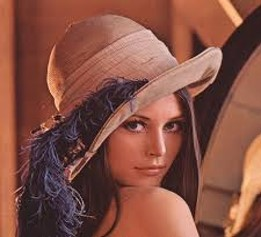
\includegraphics[width=.8\columnwidth]{fig1.jpg}
\caption{Example of a figure.}
\label{fig:ex}
\end{figure}

\textbf{Result.} a detailed description of the study results should be objectively presented, in an orderly and logical sequence using both text and illustrative materials (Tables and Figures). \\

\textbf{Discussion and Conclusions.} author's interpretation of the results, author's opinion. Conclusion should be written simply.

\subsection{Text section heading}
Divide your article into clearly defined and numbered sections. 
Subsections should be numbered as 1.1 (then 1.1.1, 1.1.2, ...), 1.2, etc. (the abstract is not included in the section numbering). 
Use this numbering also for internal cross-referencing. Any subsection may be given a brief heading. 
Each heading should appear on its own separate line.

\subsection{References in text}
References should be obviously related to documents. 
Indicate references by number(s) in square brackets in line with the text. 
The numbered references are listed in the order in which they appear in the text.
The actual authors can be referred to, but the reference number(s) must always be given. Example: '..... as demonstrated [3,6]. 
Barnaby and Jones [8] obtained a different result ....'

\subsection{Text equations}

The Equations should be punctuated and aligned to bring out their structure and numbered on the right as
\begin{equation}
y = Hx+n.
\end{equation}

Mathematical operation signs indicating continuity of the expression should be placed at the left of the second and succeeding lines. 
Use $\times$ rather than a centered dot, except for scalar products of vectors. 
The solidus ($\slash$) should be used instead of built-up fractions in running text. 
Furthermore, the Notation must be legible, clear, compact, and consistent with standard usage. 
All unusual symbols whose identity may not be obvious must be identified when they first appear, and whenever confusion might arise. 
Superscripts are normally set directly over subscripts; authors should note where readability or the meaning requires a special order. 
In the text, numbers should be Arabic numerals, except when beginning a sentence. 
Numbers greater than 999 should have commas, e.g., 13,970. 
The 24-hour system is used to indicate time, e.g., 18:00 hr. 
If you are using Word for Math, use either the Microsoft Equation Editor or the MathType add-on (\url{http://www.mathtype.com}) for equations in your paper.
“Float over text” should not be selected.

\subsection{Units and abbreviations}
Units of measure should be presented according to the International System (SI) of Units. If other units are mentioned, please give their equivalent in SI.

Abbreviations must be used as an aid to the reader, rather than as a convenience of the author, and therefore their use should be limited. 
Acronyms and abbreviations should be defined at the first time when they are used in text.

\subsection{Tables}
Each Table should be numbered with Arabic numerals in the order of their appearance in the text. 
Tables should have a concise and informative title with the table content between horizontal lines. 
The structure should be clear, with simple column headings giving all units. 
A table should not exceed one page when printed. Use lower case letters in superscripts a, b, c ... for special remarks. 
An example of a table is given in Table \ref{tab:ex}.

\subsection{Figures}
Figures are numbered consecutively in the sequence mentioned in the text and must have a caption written in one paragraph style. 
The caption should contain an explanation of all abbreviations and symbols used, and indicate the size value of lines or bars unless shown directly on the figure. 
An example of a figure is given in Fig. \ref{fig:ex}. 
The Figure number should be placed at the lower-left corner of each figure, and the numbering order must be from left to right, and from upper to lower. 
Citations of figures in the text or parentheses are abbreviated, e.g., Fig. 1, Figs. 1 and 2, Figs. 1-3, (Fig. 1), (Figs. 1 and 2), (Figs. 1-3). 
When the text refers to both figures and tables, they should be mentioned in parentheses, e.g., (Table 1; Fig. 2) and (Tables 1-3; Figs. 4-6).

\subsection{Footnotes}
Footnotes should be used sparingly. Number them consecutively throughout the article. 
Many word processors can build footnotes into the text, and this feature may be used. 
Otherwise, please indicate the position of footnotes in the text and list the footnotes themselves separately at the end of the article. 
Do not include footnotes in the Reference list.


%\section*{Acknowledgments}
%Collate acknowledgements in a separate section at the end of the article before the references and do not, therefore, include them on the title page, as a footnote to the title or otherwise.
%List here those individuals who contributed to the papers but not enough to be coauthors may be introduced. 
%Financial support, including foundations, institutions, pharmaceutical and device manufacturers, private companies, intramural departmental sources, or any other support should be described.

\section*{Appendix}
Appendix section should be placed before References section. 
If there is more than one appendix, they should be identified as A, B, etc. 
Formulae and equations in appendices should be given with separate numbering: Eq. (A.1), Eq. (A.2), etc.; in a subsequent appendix, Eq. (B.1) and so on. 
The numbering of tables and figures in the appendix is similar: Table A.1; Fig. A.1, etc.

%\section*{Conflict of interest}
%The authors declare that there is no conflict of interest in this paper.

%% References
%%
%% Following citation commands can be used in the body text:
%% Usage of \cite is as follows:
%%   \cite{key}         ==>>  [#]
%%   \cite[chap. 2]{key} ==>> [#, chap. 2]
%%

%% References with bibTeX database:

\bibliographystyle{elsarticle-num}
% \bibliographystyle{elsarticle-harv}
% \bibliographystyle{elsarticle-num-names}
% \bibliographystyle{model1a-num-names}
% \bibliographystyle{model1b-num-names}
% \bibliographystyle{model1c-num-names}
% \bibliographystyle{model1-num-names}
% \bibliographystyle{model2-names}
% \bibliographystyle{model3a-num-names}
% \bibliographystyle{model3-num-names}
% \bibliographystyle{model4-names}
% \bibliographystyle{model5-names}
% \bibliographystyle{model6-num-names}

\vspace{-0.3cm}

\begin{thebibliography}{1}

\bibitem{els} H. Kwon, K. Kim, C. Lee, The unified UE baseband modem hardware platform architecture for 3GPP specification, J. Commun. Net., 13 (1) (2011) 70-76.

\bibitem{els} T. Roos, P. Myllymaki, H. Tirri, A statistical modeling approach to location estimation, IEEE Trans. Mobile Comput. 1 (1) (2002) 59-69.

\bibitem{els} H. Liu, G. Li, OFDM-Based Broadband Wireless Networks: Design and Optimization. Hoboken, NJ: Wiley-Interscience, 2005.

\bibitem{els} T. L. Marzetta, How much training is required for multiuser MIMO?, in: 2006 Asilomar Conf. Signal. Syst. Comput., Pacific Grove, 2006, pp. 359–363.

\bibitem{els} J. Arrillaga, B. Giessner, Limitation of short-circuit levels by means of HVDC links, in: 1990 IEEE Summer Power Meeting, Los Angeles, 1990, pp. 1-8.

\bibitem{els} J. O. Williams, Narrow-band analyzer, Ph.D. dissertation, Dept. Elect. Eng., Harvard Univ., Cambridge, MA, 1993.

\bibitem{els} J. H. Davis, J. R. Cogdell, Calibration program for the 16-foot antenna, Elect. Eng. Res. Lab., Univ. Texas, Austin, Tech. Memo. NGL-006-69-3, Nov. 15, 1987.

\bibitem{els} RealVNC Ltd. Remote control software [Online]. Available: http:// www.realvnc.com


\end{thebibliography}
\end{document}

%%
%% End of file `elsarticle-template-num.tex'.
